%%%%%%%%%%%%%%%%%%%%%%%%%%%%%%%%%%%%%%%%%
% Short Sectioned Assignment
% LaTeX Template
% Version 1.0 (5/5/12)
%
% This template has been downloaded from:
% http://www.LaTeXTemplates.com
%
% Original author:
% Frits Wenneker (http://www.howtotex.com)
%
% License:
% CC BY-NC-SA 3.0 (http://creativecommons.org/licenses/by-nc-sa/3.0/)
%
% Download template:
% Overleaf (https://www.overleaf.com/8746855dtrgkbkbjjhm)
%
%%%%%%%%%%%%%%%%%%%%%%%%%%%%%%%%%%%%%%%%%

%-------------------------------------------------------------------------------
%	PACKAGES AND OTHER DOCUMENT CONFIGURATIONS
%-------------------------------------------------------------------------------

%\documentclass[paper=a4, fontsize=11pt]{scrartcl} % A4 paper and 11pt font size
\documentclass[a4paper]{article}
%\documentclass[11pt]{article}
%\usepackage[margin=1.25in]{geometry}

%\usepackage[options]{nohyperref}  % This makes hyperref commands do nothing without errors
%\usepackage{url}  % This makes \url work
%\usepackage{hyperref}

\usepackage{graphicx}

%\usepackage[T1]{fontenc} % Use 8-bit encoding that has 256 glyphs
\usepackage[utf8]{inputenc}
%\usepackage{fourier} % Use the Adobe Utopia font for the document - comment this line to return to the LaTeX default
\usepackage[english]{babel} % English language/hyphenation
\usepackage{mathtools,amsmath,amsfonts,amsthm} % Math packages
\usepackage{amssymb}

%\usepackage{lipsum} % Used for inserting dummy 'Lorem ipsum' text into the template

\usepackage{sectsty} % Allows customizing section commands
\allsectionsfont{\centering \normalfont\scshape} % Make all sections centered, the default font and small caps

\usepackage{fancyhdr} % Custom headers and footers
%\pagestyle{fancyplain} % Makes all pages in the document conform to the custom headers and footers
%\fancyhead{} % No page header - if you want one, create it in the same way as the footers below
%\fancyfoot[L]{} % Empty left footer
%\fancyfoot[C]{} % Empty center footer
%\fancyfoot[R]{\thepage} % Page numbering for right footer
\renewcommand{\headrulewidth}{0pt} % Remove header underlines
\renewcommand{\footrulewidth}{0pt} % Remove footer underlines
\setlength{\headheight}{13.6pt} % Customize the height of the header

\numberwithin{equation}{section} % Number equations within sections (i.e. 1.1, 1.2, 2.1, 2.2 instead of 1, 2, 3, 4)
\numberwithin{figure}{section} % Number figures within sections (i.e. 1.1, 1.2, 2.1, 2.2 instead of 1, 2, 3, 4)
\numberwithin{table}{section} % Number tables within sections (i.e. 1.1, 1.2, 2.1, 2.2 instead of 1, 2, 3, 4)

%\setlength\parindent{0pt} % Removes all indentation from paragraphs - comment this line for an assignment with lots of text
\usepackage{indentfirst} % Indentation for all paragraphs

% Used for definitions:
\usepackage{amsthm}
\theoremstyle{definition}
\newtheorem{definition}{Definition}[section]

% To write algorithms in pseudocode:
\usepackage{algpseudocode}
\usepackage{algorithm}

% Don't use colon in algorithms lines:
\algrenewcommand\alglinenumber[1]{\footnotesize #1}

% Input/Output instead of Require/Ensure in algorithms pseudocode:
\renewcommand{\algorithmicrequire}{\textbf{Input:}}
\renewcommand{\algorithmicensure}{\textbf{Output:}}

% To put images side by side:
\usepackage{subcaption}

% Avoid long sentences to go out of margines:
\usepackage{microtype}

% Use URL and avoid long urls to go out of margins (hyphens):
\usepackage[hyphens]{url}

% Define multiline to avoid unindented long sentences in algorithms:
% (https://tex.stackexchange.com/questions/314023/how-to-indent-a-long-sentence-in-an-algorithm)
\usepackage{tabularx}
\makeatletter
\newcommand{\multiline}[1]{%
  \begin{tabularx}{\dimexpr\linewidth-\ALG@thistlm}[t]{@{}X@{}}
    #1
  \end{tabularx}
}
\makeatother

\usepackage{tikz}
\usepackage{pgfplots}
\pgfplotsset{compat=1.15}
\usepackage{xcolor}

\definecolor{bblue}{HTML}{4F81BD}
\definecolor{rred}{HTML}{C0504D}
\definecolor{ggreen}{HTML}{9BBB59}
\definecolor{ppurple}{HTML}{9F4C7C}

\pgfplotsset{
	/pgfplots/my legend/.style={
		legend image code/.code={
			\draw[thick,black](-0.05cm,0cm) -- (0.3cm,0cm);%
		}
	}
}

%-------------------------------------------------------------------------------
%	TITLE SECTION
%-------------------------------------------------------------------------------

\newcommand{\horrule}[1]{\rule{\linewidth}{#1}} % Create horizontal rule command with 1 argument of height

\title{
\normalfont \normalsize
\textsc{Sapienza University of Rome} \\ [25pt] % Your university, school and/or department name(s)
\horrule{0.5pt} \\[0.4cm] % Thin top horizontal rule
\LARGE Neural Networks \\ % The assignment title
\large Binarized Neural Networks \\
\horrule{2pt} \\[0.5cm] % Thick bottom horizontal rule
}

\author{Ivan Bergonzani, Michele Cipriano} % Your name

\date{\normalsize\today} % Today's date or a custom date

\begin{document}
\sloppy % avoid to make words to go out of margin

\maketitle % Print the title

%-------------------------------------------------------------------------------

\section{Introduction}

The aim of the project is to implement a binarized 
neural network (BNNs), introduced in \cite{binarynet}, and test it on
the MNIST and the CIFAR-10 datasets. This new method 
introduces binary weights and activation functions in order to 
improve memory usage and replace arithmetic operations 
with bitwise operations.

The experiments achieved an accuracy on \textbf{0.961} on
MNIST and an accuracy of \textbf{0.786} on CIFAR-10
using a BNN with a shift-based Batch Normalization,
and a shift-based AdaMax optimizer.
These results are in line with
the results obtained in the original paper.

The project has been entirely developed in Python and 
TensorFlow with the exception of the GPU kernel for
the matrix multiplication that
has been developed in C++ and CUDA.

%-------------------------------------------------------------------------------

\section{BNNs}

The main characteristic of the binarized neural networks is
that the weights and the activations are constrained to +1
and -1. This makes it possible to introduce an optimized 
usage of the hardware resources when dealing with memory
management and operations on tensors. The activation function
used in this project is the Sign function, defined as:
\begin{equation*}
    x^b = \text{Sign}(x) =
        \begin{cases}
    	    +1 & \quad \text{if } x \ge 0\\
    		-1 & \quad \text{otherwise }
    	\end{cases}
\end{equation*}

Of course, since the derivative of the Sign function is zero
everywhere except at the discontinuity points, it will not
be possible to update the weights during backpropagation.
A method to solve this issue is to use the straight-through
estimator. Let's consider a cost function $C$ that depends
on a variable $q$ defined as:
\begin{equation*}
    q = \text{Sign}(r)\text{,}
\end{equation*}

\noindent when computing the partial derivative of $C$ with
respect to $r$, using the chain rule:
\begin{equation*}
    \frac{\partial C}{\partial r}
      = \frac{\partial C}{\partial q}
        \frac{\partial q}{\partial r}\text{,}
\end{equation*}

\noindent the straight-through estimator used in the paper
simply states that, given an estimator $g_q$ of
$\frac{\partial C}{\partial q}$, the estimator $g_r$ of
$\frac{\partial C}{\partial r}$ is:
\begin{equation*}
    g_r = g_q 1_{|r| \le 1}\text{,}
\end{equation*}

\noindent in this way it is possible to both preserve the
information of the gradient and to avoid gradient explosion
when $r$ becomes too large. Note that this estimation can
be obtained when propagating the gradient through the Clip
function:
\begin{gather*}
    \text{Clip}(r, -1, 1) = \text{max}(-1, \text{min}(1, r))
%\end{equation*}
%\noindent whose gradient is:
%\begin{equation*}
\\
    \frac{\partial \text{Clip}(r, -1, 1)}{\partial r}
    =
        \begin{cases}
    	    1 & \; \text{if } |r| \le 1\\
    		0 & \; \text{otherwise }
    	\end{cases}
    =
    	1_{|r| \le 1}
\end{gather*}

Hence, weights are, first, projected to values between -1
and 1
with the Clip function and are, then, binarized with the Sign
function.

Batch Normalization\cite{batchnormalization} helps to
accelerate training by reducing internal covariate shift.
This can be obtained by whitening the distribution of the
batches after each activation function of the network.
The training time can be further improved by approximating
the multiplication operations with shifting operations, using,
hence, shift-based Batch Normalization (Algorithm
\ref{algorithm:shift-based-batch-norm}). The algorithm
gets as input a batch of size $m$, computes its mean (line 2),
its variance (line 4), it normalizes (line 5), scales 
and shift (line 6) the distribution along each dimension and
returns the new minibatch $y$.

\begin{algorithm}
	\caption{Shift-based Batch Normalization\cite{binarynet}.}
	\label{algorithm:shift-based-batch-norm}
	\begin{algorithmic}[1]
	\State Let $x$ be minibatch of size $m$
	\State $\mu_B \gets \frac{1}{m} \sum_{i=1}^m x_i$
	\State $C(x_i) \gets x_i - \mu_B$
	\State $\sigma_B^2 \gets \frac{1}{m} \sum_{i=1}^m
	    (C(x_i)\ll\gg_P C(x_i))$
	\State $\hat{x}_i \gets C(x_i)\ll\gg_P (\sqrt{\sigma_B^2
	    + \epsilon})^{-1} $
	\State $y_i \gets \gamma\ll\gg_P\hat{x}_i$
	\end{algorithmic}
\end{algorithm}

Note that the
operator $\ll\gg_P$ approximates the multiplication and it is
defined as:
\begin{align*}
    \alpha \ll\gg_P \beta
        = \begin{cases}
    	    \alpha \ll +\text{round}(\text{log2}|\beta|) & \quad \text{if } \text{log2}|\beta| > 0\\
    		\alpha \gg -\text{round}(\text{log2}|\beta|) & \quad \text{otherwise} 
    	    \end{cases}
\end{align*}

\noindent similary, the operator $\ll\gg_D$ approximates the 
division and it is defined as:
\begin{align*}
    \alpha \ll\gg_D \beta
        = \begin{cases}
    	    \alpha \gg +\text{round}(\text{log2}|\beta|) & \quad \text{if } \text{log2}|\beta| > 0\\
    		\alpha \ll -\text{round}(\text{log2}|\beta|) & \quad \text{otherwise} 
    	    \end{cases}
\end{align*}

Of course, implementing these operators via hardware would 
make the computation more efficient, reducing the clock
cycles needed to complete algorithm. Note that
in our implementation, the operators $\ll\gg_P$ and
$\ll\gg_D$ have been computed by using floating point
multiplications, divisions and the approximate power of 2,
defined as
$AP2(x) = \text{sgn}(x)\times2^{\text{round}(\text{log2}
|x|)}$.

A shift-based AdaMax, based on the AdaMax implementation
introduced in \cite{adam}, has also been implemented in
order to reduce the total amount of multiplications
(Algorithm \ref{algorithm:shift-based-adamax}).
The algorithm, which
here shows the parameters update for each cycle, computes
the gradient at line 3, updates the first moment estimate
at line 4, updates the exponentially weighted infinity norm
at line 5 and then updates the parameters at line 6,
using the operators defined before.

\begin{algorithm}
	\caption{Shift-based AdaMax learning rule\cite{binarynet}.}
	\label{algorithm:shift-based-adamax}
	\begin{algorithmic}[1]
	\State Let $t$ be the current timestep, $\theta_{t-1}$
	    the parameters of the previous timestep, $f(\cdot)$ the objective function, $\beta_1,
	    \beta_2 \in [0, 1)$ exponential decay rates
	\State $t \gets t + 1$
	\State $g_t \gets \nabla_\theta f_t(\theta_{t-1})$
	\State $m_t \gets \beta_1 \cdot m_{t-1} + (1-\beta_1)
	    \cdot g_t$
	\State $u_t \gets \text{max}(\beta_2 \cdot u_{t+1},
	    |g_t|)$
	\State $\theta_t \gets \theta_{t-1} - (\alpha
	    \ll\gg_D(1-\beta_1^t)) \cdot m_t \ll\gg_D u_t$
	\end{algorithmic}
\end{algorithm}

In a binarized neural network, the binarized values of the weights
and the activations are used in the forward pass. Here, each activation
is whitened through Batch Normalization between each layer. Note that,
when training on CIFAR-10, the application of the Batch Normalization
must keep the convolutional property, hence, different elements of the same
feature map are normalized in the same way.

%In a binarized neural network, the binarized values 
%of the weights and the activations are used in the forward
%pass, as show in Algorithm \ref{algorithm:bnn-forward},
%which shows how is it 
%possible to handle continuous-valued inputs with 8 bits
%of precision (in can be generalized to whatever value $m$).
%Considering $x$ as vector of 8-bit inputs and $w^b$ a
%vector of 1-bit weights with the same size as $x$, the 
%weighted sum $s$ between $x$ and $w^b$ can be
%computed as:
%\begin{equation*}
%    s = x \cdot w^b = \sum_{n=1}^8 2^{n-1} (x^n \cdot w^b)
%\end{equation*}

%\noindent where $x^n_i$ is the n-th bit of the i-th element
%of the vector $x$.

%The algorithm simply computes the function represented by
%the network when valuated with the weights $W^b$. The 
%activations are then normalized and binarized between
%each layer, with the exception of the first one (lines 2-5),
%and the last one (lines 11-12).
%The function XnorDotProduct: TODO, C++ implementation,
%kernels, ch. 4 Seven Times Faster of GPU at Run-Time.

%\begin{algorithm}
%	\caption{Forward pass of a binarized neural network\cite{binarynet}.}
%	\label{algorithm:bnn-forward}
%	\begin{algorithmic}[1]
%	\State Let $a_0$ be a vector of 8-bit inputs, $W^b$
%	    a vector of 1-bit weights, $\theta$ the parameters
%	    of the Batch Normalization algorithm, and $L$ the 
%	    number of layers of the network.
%	\State $a_1 \gets 0$ 
%	\For {$n=1$ to 8}
%	    \State $a_1 \gets a_1 + 2^{n-1} \times 
%	        \text{XnorDotProduct}(a_0^n, W_1^b)$
%	\EndFor
%	\State $a_1^b \gets
%	    \text{Sign}(\text{BatchNorm}(a_1, \theta_1))$
%	\For {$k=2$ to $L-1$}
%	    \State $a_k \gets \text{XnorDotProduct}(a_{k-1}^b,
%	        W_k^b)$
%	    \State $a_k^b \gets
%	        \text{Sign}(\text{BatchNorm}(a_k, \theta_k))$
%	\EndFor
%	\State $a_L \gets \text{XnorDotProduct}(a_{L-1}^b,
%	        W_L^b)$
%    \State $a_L \gets \text{BatchNorm}(a_L, \theta_L)$
%	\end{algorithmic}
%\end{algorithm}

\section{Experiments}

The model has been tested on the datasets MNIST and CIFAR-10
comparing three different DNNs:
\begin{itemize}
    \item A standard deep neural network with ReLU
        nonlinearity, the original implementation of
        Batch Normalization
        (\texttt{tf.layers.batch\_normalization})
        and a vanilla implementation of ADAM
        (\texttt{tf.optimizers.AdamOptimizer}) as optimizer
    \item A binarized neural network with the Sign function
        for nonlinearity, the original implementation of
        Batch Normalization and a vanilla implementation of ADAM
        (\texttt{tf.optimizers.AdamOptimizer}) as optimizer
    \item A binarized neural network with the Sign function
        for nonlinearity, a shifted-based implementation
        of Batch Normalization and a shifted-based
        implementation of AdaMax
\end{itemize}

On the dataset MNIST, the networks have been trained for 20
epochs with a batch size of 100, while, on the dataset
CIFAR-10, the networks have been trained for 50 epochs
with a batch size of 50. For both datasets the learning
rate has been initially set to 0.001 and divided by 2
after each 10 epochs (which could be obtained by
shifting the bits to the right by 1). All the
experiments used the cross entropy as loss function.

As it is possible to see from table \ref{table:experiments},
on the dataset MNIST, the networks achieved an accuracy of \textbf{0.984} on the
test set when
using the ReLU activation function, the Batch Normalization implementation
of TensorFlow and the ADAM optimizer, \textbf{0.984} when using the Sign 
activation function, the Batch Normalization implementation of TensorFlow
and the ADAM optimizer, and \textbf{0.961} when using the Sign
activation function,
and a binarized implementation of both Batch Normalization and AdaMax
optimizer. On the dataset CIFAR-10, the networks achieved an accuracy
of \textbf{0.884} on the test set when
using the ReLU activation function, the Batch Normalization implementation
of TensorFlow and the ADAM optimizer, \textbf{0.784} when using the Sign 
activation function, the Batch Normalization implementation of TensorFlow
and the ADAM optimizer, and \textbf{0.786} when using the Sign activation
function,
and a binarized implementation of both Batch Normalization and AdaMax
optimizer.

The experiments have been performed on Google Compute Engine
using an NVIDIA Tesla K80 to speed up the training.

\begin{table}
	\centering
	\begin{tabular}{*{5}{c}}
		Network & Batch Norm. & Dataset & Train Acc. & Test. Acc. \\
		\hline
		Standard & Standard & MNIST & 1.000 & 0.984 \\
		Binarized & Standard & MNIST & 0.999 & 0.984 \\
		Binarized & Shift-based & MNIST & 0.965 & 0.961 \\
		\hline
		Standard & Standard & CIFAR-10 & 1.000 & 0.884 \\
		Binarized & Standard & CIFAR-10 & 0.999 & 0.784 \\
		Binarized & Shift-based & CIFAR-10 & 0.897 & 0.786 \\
	\end{tabular}
	\caption{
	    The table shows the results of the experiments.
	    A network can either be ``Standard'' or ``Binarized'',
	    in the latter case the weights and the activation 
	    functions are binarized. Similarly, Batch Normalization
	    can be ``Standard'' if implemented as in the original
	    paper\cite{batchnormalization} or ``Shift-based'' if
	    it makes use of shift operators in order to exploit
	    hardware implementations. Binarized networks with
	    shift-based batch normalization makes use of a
	    shift-based implementation of AdaMax as optimizer,
	    while all the other experiments use a vanilla
	    implementation of ADAM.}
    \label{table:experiments}
\end{table}

\begin{figure}
    \centering
    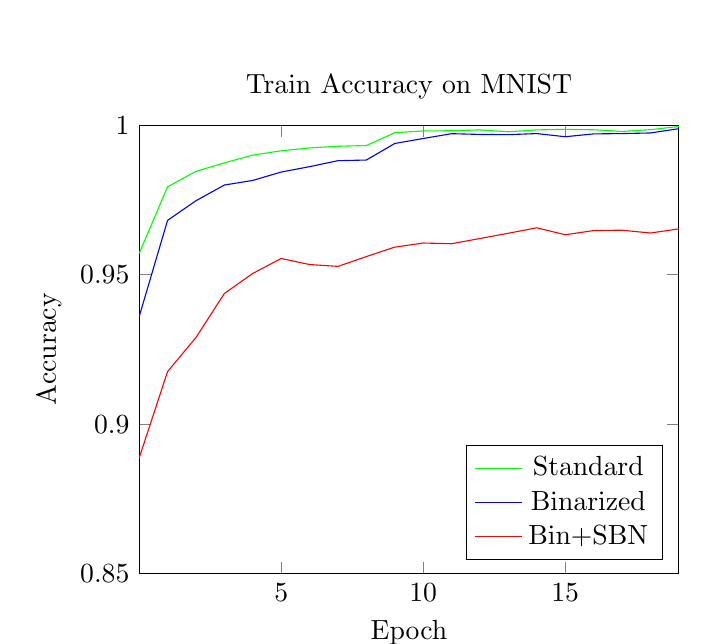
\begin{tikzpicture}
        \begin{axis}[
            title={Train Accuracy on MNIST},
            xlabel={Epoch},
            ylabel={Accuracy},
            xmin=0, xmax=19,
            ymin=0.85, ymax=1,
            xtick={5,10,15},
            ytick={0.85,0.9,0.95,1.0},
            legend pos=south east,
            %ymajorgrids=true,
            %grid style=dashed,
        ]
            
            \addplot[color=green]
            coordinates{
                (0, 0.9570909142494202) (1, 0.9793999791145325) (2, 0.9845454692840576) (3, 0.9873999953269958) (4, 0.9900000095367432) (5, 0.9914363622665405) (6, 0.9923999905586243) (7, 0.9929454326629639) (8, 0.9932000041007996) (9, 0.9974908828735352) (10, 0.9980727434158325) (11, 0.9981454610824585) (12, 0.9984181523323059) (13, 0.9977999925613403) (14, 0.9984363913536072) (15, 0.9986000061035156) (16, 0.9984727501869202) (17, 0.9979090690612793) (18, 0.9985091090202332) (19, 0.9995636343955994) 
            };
            \addlegendentry{Standard}
            
            \addplot[color=blue]
            coordinates{
                (0, 0.935945451259613) (1, 0.9681636095046997) (2, 0.9747272729873657) (3, 0.9799818396568298) (4, 0.9815272688865662) (5, 0.9843272566795349) (6, 0.9861272573471069) (7, 0.9881272912025452) (8, 0.9883454442024231) (9, 0.9938908815383911) (10, 0.9955454468727112) (11, 0.9971636533737183) (12, 0.9969090819358826) (13, 0.9968363642692566) (14, 0.9972000122070312) (15, 0.9961454272270203) (16, 0.9970909357070923) (17, 0.9972000122070312) (18, 0.9973999857902527) (19, 0.99883633852005) 
            };
            \addlegendentry{Binarized}
            
            \addplot[color=red]
            coordinates{
                (0, 0.8886545300483704) (1, 0.9175636172294617) (2, 0.9289636611938477) (3, 0.9436908960342407) (4, 0.9503999948501587) (5, 0.9553999900817871) (6, 0.9533818364143372) (7, 0.9527636170387268) (8, 0.956036388874054) (9, 0.9592000246047974) (10, 0.9605818390846252) (11, 0.960345447063446) (12, 0.9620909094810486) (13, 0.9638545513153076) (14, 0.9656727313995361) (15, 0.963345468044281) (16, 0.9647454619407654) (17, 0.9648727178573608) (18, 0.9639272689819336) (19, 0.9653090834617615) 
            };
            \addlegendentry{Bin+SBN}
            
        \end{axis}

    \end{tikzpicture}
    \caption{The plot shows the how the train accuracy
        varies for the dataset MNIST using standard
        activations, binary activations and binary
        activations with shift-based
        Batch Normalization.}
    \label{fig:train-accuracy-mnist}
\end{figure}

\begin{figure}
    \centering
    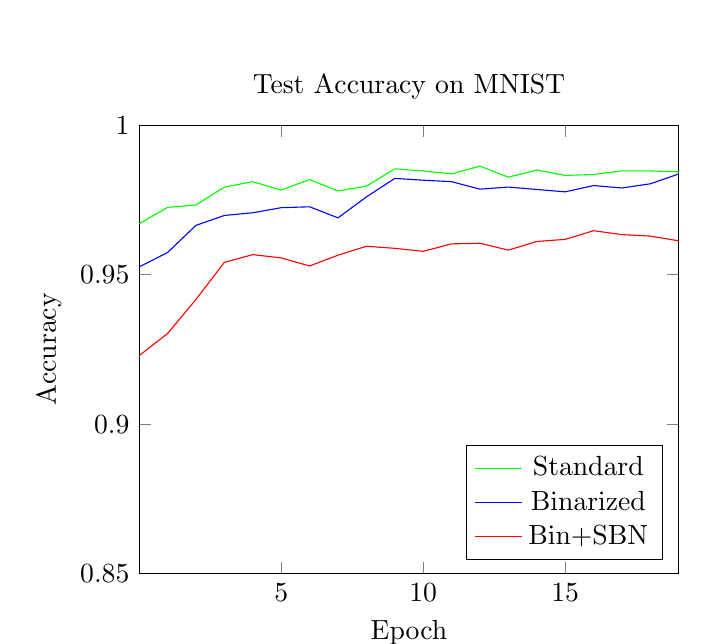
\begin{tikzpicture}
        \begin{axis}[
            title={Test Accuracy on MNIST},
            xlabel={Epoch},
            ylabel={Accuracy},
            xmin=0, xmax=19,
            ymin=0.85, ymax=1,
            xtick={5,10,15},
            ytick={0.85,0.9,0.95,1.0},
            legend pos=south east,
            %ymajorgrids=true,
            %grid style=dashed,
        ]
            
            \addplot[color=green]
            coordinates{
                (0, 0.9670000076293945) (1, 0.9725000262260437) (2, 0.9732999801635742) (3, 0.9793000221252441) (4, 0.9811000227928162) (5, 0.9782999753952026) (6, 0.9818000197410583) (7, 0.9779999852180481) (8, 0.9796000123023987) (9, 0.9854000210762024) (10, 0.9847000241279602) (11, 0.9836999773979187) (12, 0.986299991607666) (13, 0.9825999736785889) (14, 0.9850000143051147) (15, 0.9832000136375427) (16, 0.9835000038146973) (17, 0.9847000241279602) (18, 0.9847000241279602) (19, 0.9843999743461609) 
            };
            \addlegendentry{Standard}
            
            \addplot[color=blue]
            coordinates{
                (0, 0.9526000022888184) (1, 0.9574000239372253) (2, 0.9664999842643738) (3, 0.9697999954223633) (4, 0.9707000255584717) (5, 0.9724000096321106) (6, 0.9726999998092651) (7, 0.968999981880188) (8, 0.9760000109672546) (9, 0.982200026512146) (10, 0.9815999865531921) (11, 0.9811000227928162) (12, 0.978600025177002) (13, 0.9793000221252441) (14, 0.9785000085830688) (15, 0.9776999950408936) (16, 0.9797999858856201) (17, 0.9789999723434448) (18, 0.980400025844574) (19, 0.9836999773979187) 
            };
            \addlegendentry{Binarized}
            
            \addplot[color=red]
            coordinates{
                (0, 0.9229000210762024) (1, 0.9302999973297119) (2, 0.9416999816894531) (3, 0.9541000127792358) (4, 0.9567000269889832) (5, 0.9556000232696533) (6, 0.9528999924659729) (7, 0.9564999938011169) (8, 0.9595000147819519) (9, 0.9588000178337097) (10, 0.9577999711036682) (11, 0.9603000283241272) (12, 0.9605000019073486) (13, 0.9581999778747559) (14, 0.9610999822616577) (15, 0.9617999792098999) (16, 0.9646999835968018) (17, 0.9634000062942505) (18, 0.9628999829292297) (19, 0.9613000154495239)  
            };
            \addlegendentry{Bin+SBN}
            
        \end{axis}

    \end{tikzpicture}
    \caption{The plot shows the how the test accuracy
        varies for the dataset MNIST using standard
        activations, binary activations and binary
        activations with shift-based
        Batch Normalization.}
    \label{fig:test-accuracy-mnist}
\end{figure}

\begin{figure}
    \centering
    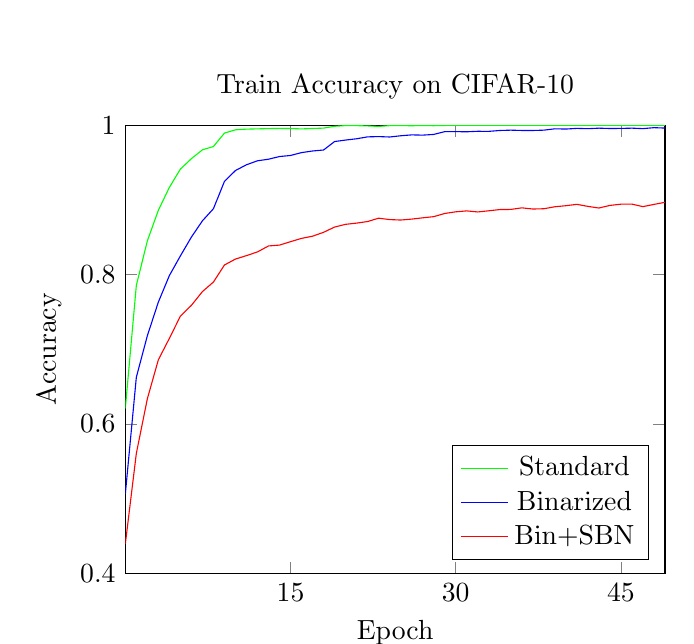
\begin{tikzpicture}
        \begin{axis}[
            title={Train Accuracy on CIFAR-10},
            xlabel={Epoch},
            ylabel={Accuracy},
            xmin=0, xmax=49,
            ymin=0.4, ymax=1,
            xtick={15,30,45},
            ytick={0.4,0.6,0.8,1.0},
            legend pos=south east,
            %ymajorgrids=true,
            %grid style=dashed,
        ]
            
            \addplot[color=green]
            coordinates{
                (0, 0.6208800077438354) (1, 0.7856199741363525) (2, 0.8451799750328064) (3, 0.8861600160598755) (4, 0.9168000221252441) (5, 0.9412400126457214) (6, 0.9552199840545654) (7, 0.9670400023460388) (8, 0.9714999794960022) (9, 0.9894400238990784) (10, 0.9938200116157532) (11, 0.9947400093078613) (12, 0.9951000213623047) (13, 0.9954599738121033) (14, 0.9956799745559692) (15, 0.9955199956893921) (16, 0.9950600266456604) (17, 0.9955800175666809) (18, 0.9961000084877014) (19, 0.9985799789428711) (20, 0.999459981918335) (21, 0.9994199872016907) (22, 0.9990400075912476) (23, 0.9983800053596497) (24, 0.9994199872016907) (25, 0.999459981918335) (26, 0.9992799758911133) (27, 0.9995200037956238) (28, 0.9993199706077576) (29, 0.9996600151062012) (30, 0.9998000264167786) (31, 0.9998999834060669) (32, 0.999779999256134) (33, 0.9998000264167786) (34, 0.9998999834060669) (35, 0.9999399781227112) (36, 0.9999399781227112) (37, 0.9999799728393555) (38, 0.9998400211334229) (39, 0.9999399781227112) (40, 0.9999799728393555) (41, 1.0) (42, 0.9999799728393555) (43, 0.9999600052833557) (44, 1.0) (45, 0.9999799728393555) (46, 1.0) (47, 1.0) (48, 1.0) (49, 0.9999799728393555) 
            };
            \addlegendentry{Standard}
            
            \addplot[color=blue]
            coordinates{
                (0, 0.5064200162887573) (1, 0.6626999974250793) (2, 0.7182599902153015) (3, 0.7633200287818909) (4, 0.7987800240516663) (5, 0.8250799775123596) (6, 0.8502799868583679) (7, 0.8720399737358093) (8, 0.8882200121879578) (9, 0.924780011177063) (10, 0.9393200278282166) (11, 0.9470599889755249) (12, 0.9523800015449524) (13, 0.9545000195503235) (14, 0.9580600261688232) (15, 0.9595000147819519) (16, 0.9633200168609619) (17, 0.9654800295829773) (18, 0.9667999744415283) (19, 0.9781200289726257) (20, 0.9801200032234192) (21, 0.9818400144577026) (22, 0.9843999743461609) (23, 0.9847599864006042) (24, 0.984220027923584) (25, 0.9858599901199341) (26, 0.9870399832725525) (27, 0.9867200255393982) (28, 0.9876400232315063) (29, 0.991320013999939) (30, 0.9914000034332275) (31, 0.9911999702453613) (32, 0.9918599724769592) (33, 0.9917600154876709) (34, 0.9929199814796448) (35, 0.9933599829673767) (36, 0.9929599761962891) (37, 0.9929199814796448) (38, 0.9933599829673767) (39, 0.9951800107955933) (40, 0.9948400259017944) (41, 0.9957399964332581) (42, 0.9953399896621704) (43, 0.9960200190544128) (44, 0.9955800175666809) (45, 0.9957000017166138) (46, 0.9960399866104126) (47, 0.995419979095459) (48, 0.9966999888420105) (49, 0.99617999792099) 
            };
            \addlegendentry{Binarized}
            
            \addplot[color=red]
            coordinates{
                (0, 0.439520001411438) (1, 0.5608000159263611) (2, 0.6338800191879272) (3, 0.6860799789428711) (4, 0.714739978313446) (5, 0.7444599866867065) (6, 0.7589200139045715) (7, 0.7773000001907349) (8, 0.7900800108909607) (9, 0.8128799796104431) (10, 0.8208400011062622) (11, 0.8254600167274475) (12, 0.8304200172424316) (13, 0.838379979133606) (14, 0.8395599722862244) (15, 0.8440999984741211) (16, 0.8485199809074402) (17, 0.8514599800109863) (18, 0.8566399812698364) (19, 0.8636599779129028) (20, 0.8673400282859802) (21, 0.8689600229263306) (22, 0.8710799813270569) (23, 0.875540018081665) (24, 0.8736799955368042) (25, 0.8730800151824951) (26, 0.8743199706077576) (27, 0.876039981842041) (28, 0.8776000142097473) (29, 0.8818600177764893) (30, 0.8840799927711487) (31, 0.8853200078010559) (32, 0.883899986743927) (33, 0.8854399919509888) (34, 0.8870999813079834) (35, 0.8872799873352051) (36, 0.8894000053405762) (37, 0.8878200054168701) (38, 0.8881800174713135) (39, 0.8908399939537048) (40, 0.8922600150108337) (41, 0.8940799832344055) (42, 0.8913599848747253) (43, 0.8891599774360657) (44, 0.8926399946212769) (45, 0.8942800164222717) (46, 0.8943799734115601) (47, 0.8910199999809265) (48, 0.8939999938011169) (49, 0.8967800140380859)  
            };
            \addlegendentry{Bin+SBN}
            
        \end{axis}

    \end{tikzpicture}
    \caption{The plot shows the how the train accuracy
        varies for the dataset CIFAR-10 using standard
        activations, binary activations and binary
        activations with shift-based
        Batch Normalization.}
    \label{fig:train-accuracy-cifar10}
\end{figure}

\begin{figure}
    \centering
    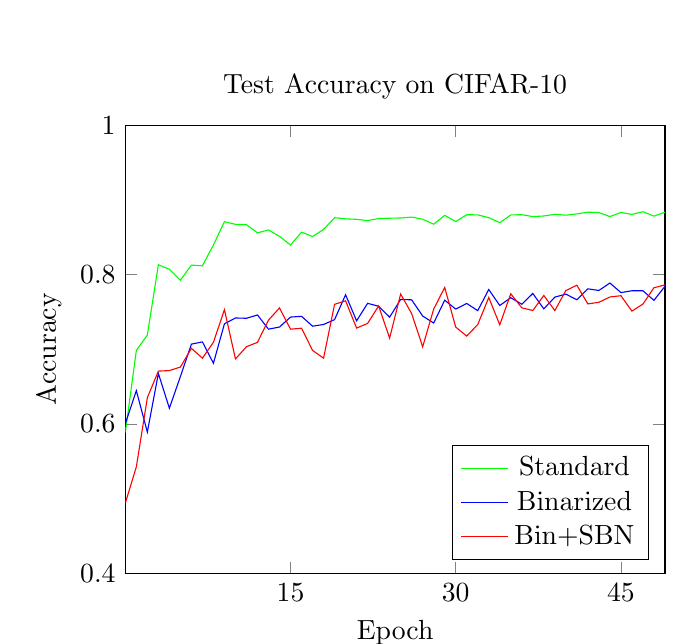
\begin{tikzpicture}
        \begin{axis}[
            title={Test Accuracy on CIFAR-10},
            xlabel={Epoch},
            ylabel={Accuracy},
            xmin=0, xmax=49,
            ymin=0.4, ymax=1,
            xtick={15,30,45},
            ytick={0.4,0.6,0.8,1.0},
            legend pos=south east,
            %ymajorgrids=true,
            %grid style=dashed,
        ]
            
            \addplot[color=green]
            coordinates{
                (0, 0.588699996471405) (1, 0.6985999941825867) (2, 0.7190999984741211) (3, 0.8131999969482422) (4, 0.807200014591217) (5, 0.7925999760627747) (6, 0.8126999735832214) (7, 0.8119000196456909) (8, 0.8396999835968018) (9, 0.8708999752998352) (10, 0.8672999739646912) (11, 0.8668000102043152) (12, 0.8560000061988831) (13, 0.8597999811172485) (14, 0.8513000011444092) (15, 0.8396000266075134) (16, 0.8568999767303467) (17, 0.8510000109672546) (18, 0.8604999780654907) (19, 0.8762000203132629) (20, 0.8747000098228455) (21, 0.8740000128746033) (22, 0.8723000288009644) (23, 0.8751000165939331) (24, 0.8755000233650208) (25, 0.8758000135421753) (26, 0.8769999742507935) (27, 0.8741999864578247) (28, 0.8675000071525574) (29, 0.8792999982833862) (30, 0.8709999918937683) (31, 0.8802000284194946) (32, 0.8799999952316284) (33, 0.8762999773025513) (34, 0.8694999814033508) (35, 0.8798999786376953) (36, 0.8802000284194946) (37, 0.8776999711990356) (38, 0.8784999847412109) (39, 0.8808000087738037) (40, 0.8795999884605408) (41, 0.8812999725341797) (42, 0.8835999965667725) (43, 0.8830999732017517) (44, 0.8776999711990356) (45, 0.8831999897956848) (46, 0.8805999755859375) (47, 0.8841999769210815) (48, 0.8783000111579895) (49, 0.8834999799728394)  
            };
            \addlegendentry{Standard}
            
            \addplot[color=blue]
            coordinates{
                (0, 0.6007000207901001) (1, 0.6446999907493591) (2, 0.5892999768257141) (3, 0.6678000092506409) (4, 0.6212000250816345) (5, 0.6636000275611877) (6, 0.7070000171661377) (7, 0.7099999785423279) (8, 0.6814000010490417) (9, 0.7342000007629395) (10, 0.7419999837875366) (11, 0.741599977016449) (12, 0.7459999918937683) (13, 0.7269999980926514) (14, 0.7299000024795532) (15, 0.7432000041007996) (16, 0.7441999912261963) (17, 0.7310000061988831) (18, 0.733299970626831) (19, 0.739799976348877) (20, 0.7731000185012817) (21, 0.7382000088691711) (22, 0.7616000175476074) (23, 0.7577000260353088) (24, 0.7430999875068665) (25, 0.7667999863624573) (26, 0.7663000226020813) (27, 0.7445999979972839) (28, 0.7351999878883362) (29, 0.7657999992370605) (30, 0.7538999915122986) (31, 0.7613999843597412) (32, 0.751800000667572) (33, 0.7800999879837036) (34, 0.7587000131607056) (35, 0.76910001039505) (36, 0.7603999972343445) (37, 0.7748000025749207) (38, 0.7541999816894531) (39, 0.7699000239372253) (40, 0.7738999724388123) (41, 0.7663999795913696) (42, 0.781000018119812) (43, 0.7788000106811523) (44, 0.7888000011444092) (45, 0.7760000228881836) (46, 0.7784000039100647) (47, 0.7784000039100647) (48, 0.7656000256538391) (49, 0.7843999862670898)
            };
            \addlegendentry{Binarized}
            
            \addplot[color=red]
            coordinates{
                (0, 0.4941999912261963) (1, 0.5428000092506409) (2, 0.6353999972343445) (3, 0.6708999872207642) (4, 0.6715999841690063) (5, 0.6762999892234802) (6, 0.7013999819755554) (7, 0.6881999969482422) (8, 0.7095000147819519) (9, 0.7530999779701233) (10, 0.6872000098228455) (11, 0.703499972820282) (12, 0.7093999981880188) (13, 0.7391999959945679) (14, 0.7554000020027161) (15, 0.7269999980926514) (16, 0.7282999753952026) (17, 0.6985999941825867) (18, 0.6881999969482422) (19, 0.7602999806404114) (20, 0.7649000287055969) (21, 0.7285000085830688) (22, 0.7347000241279602) (23, 0.7580999732017517) (24, 0.7149999737739563) (25, 0.7739999890327454) (26, 0.7479000091552734) (27, 0.7034000158309937) (28, 0.7538999915122986) (29, 0.7828999757766724) (30, 0.7297999858856201) (31, 0.7178000211715698) (32, 0.7332000136375427) (33, 0.7694000005722046) (34, 0.7328000068664551) (35, 0.774399995803833) (36, 0.7555999755859375) (37, 0.7519999742507935) (38, 0.7720999717712402) (39, 0.7519000172615051) (40, 0.7786999940872192) (41, 0.7857999801635742) (42, 0.7608000040054321) (43, 0.7630000114440918) (44, 0.7700999975204468) (45, 0.7717999815940857) (46, 0.7512000203132629) (47, 0.7605999708175659) (48, 0.7825000286102295) (49, 0.7861999869346619) 
            };
            \addlegendentry{Bin+SBN}
            
        \end{axis}

    \end{tikzpicture}
    \caption{The plot shows the how the test accuracy
        varies for the dataset CIFAR-10 using standard
        activations, binary activations and binary
        activations with shift-based
        Batch Normalization.}
    \label{fig:test-accuracy-cifar10}
\end{figure}

The forward pass of a binarized neural network could be further optimized
by using a kernel that exploits operators that are already implemented on
hardware. In our implementation a GPU kernel for the matrix multiplication
has been developed in order to test how the use of XNOR operator could
speed up the computation with respect to the original TensorFlow implementation
of \texttt{tf.matmul}.
Since, in a BNN, the matrices which represent the weights and activations are binary, it is possible to store the single values into bits by concatenating the rows of the left operand and the columns of the right operand into integers. In this way it is possible to group 32/64 elements into the 32/64 bit of a single integer.
Once the two matrices have been obtained, the rows-columns multiplication problem is reduced to a compositions of the bitwise operations popcount\footnote{popcount returns the number of bit in a number}, xnor and an accumulator of their result:
\begin{equation*}
	b_{cnt} = \sum_{1}^{n}\text{popcount}(\text{xnor}(a_{rj}, w_{jc}))
\end{equation*}
\begin{equation*}
	y_{rc} = b_{cnt} - (m - b_{cnt})
\end{equation*}
where $m$ is the length of row $r$ and column $c$. Value $n$ represents instead the number of integer needed to store their binary values.

The matrices concatenations and multiplication kernels have been developed in C++ with the use of CUDA libraries and it have been tested on Google Compute Engine with an NVIDIA Tesla K80.

Figure \ref{fig:matmul-time} shows the time needed to perform a matrix
multiplication with different kernels changing the size of the matrices
themselves. Here, it is possible to see that our implementation is faster
than the original TensorFlow implementation.

\begin{figure}
	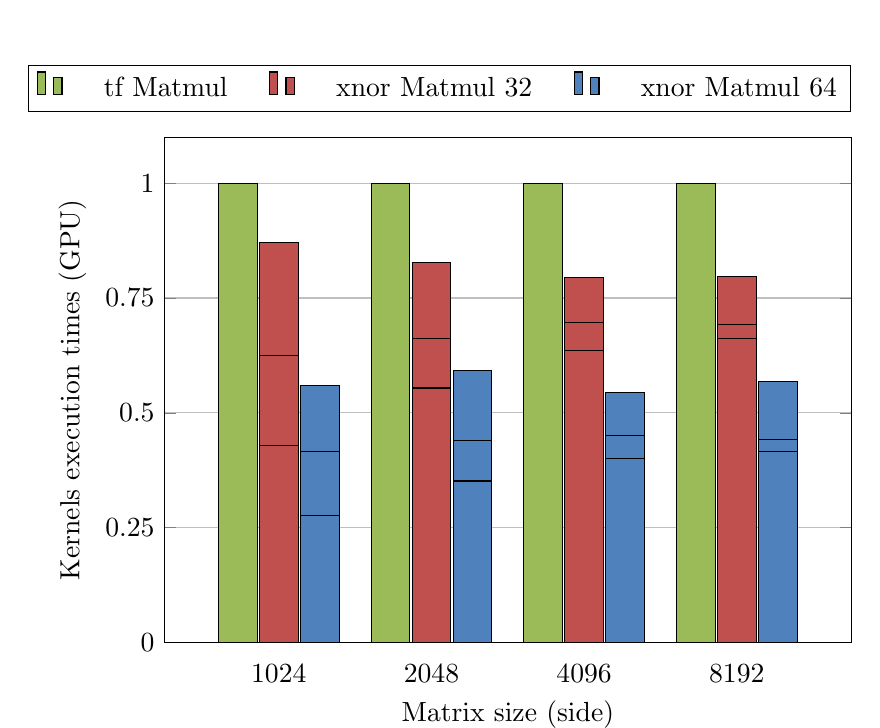
\begin{tikzpicture}
	\begin{axis}[
	width  = 0.85*\textwidth,
	height = 8cm,
	major x tick style = transparent,
	ybar=2*\pgflinewidth,
	bar width=14pt,
	ymajorgrids = true,
	xlabel = {Matrix size (side)},
	ylabel = {Kernels execution times (GPU)},
	symbolic x coords={1024,2048,4096,8192,8192ncc,ncc},
	ytick = {0, 0.25, 0.5, 0.75, 1},
	xtick = data,
	scaled y ticks = false,
	enlarge x limits=0.25,
	ymin=0,
	legend cell align=left,
	legend columns=3,
	legend style={
		at={(1,1.05)},
		anchor=south east,
		column sep=3ex
	},
	extra y tick labels={},
	extra y tick style={grid=major,major grid style={thick,draw=black}}
	]
	%\addplot[style={bblue,fill=bblue,mark=none}]
	%coordinates {(1024, 1.456) (2048,8.966) (4096,64.288) (8192,495.732)};
	
	%\addplot[style={rred,fill=rred,mark=none}]
	%coordinates {(1024,1.267) (2048,7.425) (4096,51.104) (8192,395.183)};
	
	%\addplot[style={ggreen,fill=ggreen,mark=none}]
	%coordinates {(1024,0.815) (2048,5.311) (4096,35.036) (8192,281.661)};
	
	%\addplot[style={black,fill=ggreen,mark=none}]
	%coordinates {(8192,495.732) (8192,495.732) (8192ncc,495.732)};
	
	%\addplot[style={black,fill=rred,mark=none}]
	%coordinates {(8192,395.183) (8192,343.238) (8192,327.811)   (8192ncc,343.238) (8192ncc,327.811)};
	
	%\addplot[style={black,fill=bblue,mark=none}]
	%coordinates {(8192,281.661) (8192,218.666) (8192,206.088)   (8192ncc,218.666) (8192ncc,206.088)};
	
	% standard tf mult
	\addplot[style={black,fill=ggreen,mark=none}]
	coordinates {(1024,1) (2048,1) (4096,1) (8192,1)};
	
	% xnor matmul 32
	\addplot[style={black,fill=rred,mark=none}]
	coordinates {(1024,0.8702) (1024,0.625) (1024,0.4299)
		(2048,0.8281) (2048,0.6620) (2048,0.5540)
		(4096,0.7949) (4096,0.6962) (4096,0.6360)
		(8192,0.797) (8192,0.6923) (8192,0.6612)};
	
	%xnor matmul 64
	\addplot[style={black,fill=bblue,mark=none}]
	coordinates {(1024,0.5597) (1024,0.4162) (1024,0.2761)
		(2048,0.5923) (2048,0.4405) (2048,0.3517)
		(4096,0.5449) (4096,0.4506) (4096,0.4015)
		(8192,0.5681) (8192,0.4411) (8192,0.4157)};
	
	\legend{tf Matmul, xnor Matmul 32, xnor Matmul 64}
	
	\end{axis}
	\end{tikzpicture}
	\caption{The figure shows the relationship between
		the execution time of \texttt{tf.matmul} and our
		matrix multiplication kernels which use the
		XNOR operator on 32 and 64 bits. The columns
		representing these last two kernel are divided
		in three parts, the concatenate columns operation
		on the top, the concatenate rows in the middle
		and the actual matrix multiplication
		on the bottom.}
	\label{fig:matmul-time}
\end{figure}

The implemented xnor matmul has been tested also on the forward propagation of a multilayer perceptron with 1024 input nodes, 3 hidden dense layers of 4096 nodes and an output layer of 10 nodes. The hidden dense layers were implemented using the xnor multiplication followed by a sign activation. 
This network was compared against a similar one which used only the vanilla tensorflow matmul on the evaluation of a dataset with around 60000 entries.

These results are
highlighted on table \ref{table:fp-exec-time} which shows the
relationship between the execution times of the different kernels,
grouped with respect to the size of the batches.

A further advantage is given by the fact that during inference the weight matrices are fixed and their columns concatenation can be done just once at initialization time.

\begin{table}
	\centering
	\begin{tabular}{c|*{5}{c}}
		& \multicolumn{5}{c}{batch size} \\
		kernel & 8192 & 4096 & 2048 & 1024 & 512 \\
		\hline
		\texttt{tf.matmul} & 2.623 & 2.504 & 2.718 & 2.832 & 3.252 \\
		\texttt{xnor32} & 2.142 & 2.137 & 2.417 & 2.783 & 3.785 \\
		\texttt{xnor64} & 1.707 & 1.687 & 1.958 & 2.303 & 3.288 \\
	\end{tabular}
	\caption{
	    The table shows the execution time (in seconds) of different multiplication kernels  on the forward propagation over a dataset with around 60000 entries. \texttt{tf} is the TensorFlow
	    implementation, \texttt{xnor32} is the implementation using our kernel with
	    32 bits while \texttt{xnor64} is the implementation using
	    our kernel with 64 bits.}
    \label{table:fp-exec-time}
\end{table}


%-------------------------------------------------------------------------------

\section{Conclusions}

Binarized Neural Networks promise to speed up the training phase by
exploiting hardware implementation, which becomes possible because
of the use of binary weights and activation functions. Moreover, since
multiplications and division are much harder to implement
than shifting, BNNs would use less power. Finally, working on
bits allows to reduce the amount of memory needed in the 
networks, resulting in a smaller number of memory accesses
which would further speed up the computation and reduce
the power consumption.

The implementation of a GPU kernel for the matrix multiplication
using the XNOR operator showed how it could be possible to reduce the
training time when using binarized values. Notice that this could
be improved even more by fusing the hardware instructions altogether.

Our implementation reflects the results presented in the paper,
achieving good results in both MNIST and CIFAR-10 datasets.
Of course, due to the unavailability of the GPU resources it
has not been possible to identically reproduce the experiments
of the authors.

%-------------------------------------------------------------------------------

\newpage
\bibliography{bibliography}
\bibliographystyle{ieeetr}

%-------------------------------------------------------------------------------

\end{document}
\grid
\grid
